\documentclass{beamer}
%
% Choose how your presentation looks.
% For more themes, color themes and font themes, see:
% http://deic.uab.es/~iblanes/beamer_gallery/index_by_theme.html
%
\mode<presentation>
{
  \usetheme{Madrid}      % or try Darmstadt, Madrid, Warsaw, ...
  \usecolortheme{seahorse} % or try albatross, beaver, crane, ...
  \usefonttheme{serif}  % or try serif, structurebold, ...
  \setbeamertemplate{navigation symbols}{}
  \setbeamertemplate{caption}[numbered]
  \usepackage{amsmath}
  \usepackage{tcolorbox}
  \usepackage[export]{adjustbox}
  \tcbuselibrary{most}
  \usepackage{arydshln}
  \usepackage{tikz}
  \usetikzlibrary{plotmarks}
  \usepackage{pgfplots}
   \usepackage{hyperref}
   
\setbeamercolor*{enumerate item}{bg=red,fg=black}
\setbeamercolor*{enumerate subitem}{bg=red,fg=black}
\setbeamercolor*{enumerate subsubitem}{bg=red,fg=black}
} 


\definecolor{myblue}{RGB}{65,105,225} 
\definecolor{myorange}{RGB}{250,190,0}

\setbeamercolor{structure}{fg=white,bg=myorange}
\setbeamercolor*{palette primary}{fg=myblue,bg=myorange}
\setbeamercolor*{palette secondary}{fg=white,bg=myblue}
\setbeamercolor*{palette tertiary}{bg=myblue,fg=white}
\setbeamercolor*{palette quaternary}{fg=white,bg=myorange!50}

\setbeamercolor{frametitle}{fg=black!90!myblue}

\setbeamercolor{section in head/foot}{fg=white,bg=myblue}
\setbeamercolor{author in head/foot}{fg=black,bg=myorange}
\setbeamercolor{title in head/foot}{fg=white,bg=myblue}

\setbeamertemplate{navigation symbols}{}

\setbeamertemplate{itemize/enumerate body begin}{\large}
\setbeamertemplate{itemize/enumerate subbody begin}{\large}
\setbeamertemplate{itemize/enumerate subsubbody begin}{\large}
\setbeamertemplate{itemize/enumerate subsubsubbody begin}{\large}



\defbeamertemplate*{headline}{mytheme}
{%
  \begin{beamercolorbox}[ht=2.25ex,dp=3.75ex]{section in head/foot}
    \insertnavigation{\paperwidth}
  \end{beamercolorbox}%
}%

\defbeamertemplate*{footline}{mytheme}
{
  \leavevmode%
  \hbox{%
  \begin{beamercolorbox}[wd=.5\paperwidth,ht=2.25ex,dp=1ex,right]{author in head/foot}%
    \usebeamerfont{author in head/foot}\insertshortauthor\hspace*{2em}
  \end{beamercolorbox}%
  \begin{beamercolorbox}[wd=.5\paperwidth,ht=2.25ex,dp=1ex,left]{title in head/foot}%
    \usebeamerfont{title in head/foot}\hspace*{2em}\insertshortsubtitle\hspace*{2em}
    \insertframenumber{} / \inserttotalframenumber
  \end{beamercolorbox}}%
  \vskip0pt%
}



\usepackage[english]{babel}
%\usepackage[utf8x]{inputenc}
\usepackage{xcolor}
\definecolor{light-cyan}{cmyk}{0.25,0,0,0}
\usepackage{listings}
      % For listings https://tex.stackexchange.com/questions/180222/how-to-change-font-size-for-specific-lstlisting
      % https://tex.stackexchange.com/questions/119863/problems-with-the-lstlisting-environment-margin-and-white-line
  \lstdefinestyle{myPythonStyle}{
    language=Python,
    numbersep=10pt,
    tabsize=4,
    showspaces=false,
   showstringspaces=false,
   backgroundcolor=\color{light-cyan},
   xleftmargin=0.5cm,
   frame=lr,
   framesep=8pt,
   framerule=0pt
}

\usepackage{pgf}  
\usepackage{textpos}
\usepackage{tabulary}
\usepackage{scrextend}
\usepackage{hyperref}
\usepackage{setspace}
\usepackage{rotating}
\lstset
{
    language=[LaTeX]TeX,
    breaklines=true,
    basicstyle=\tt\scriptsize,
    %commentstyle=\color{green}
    keywordstyle=\color{blue},
    %stringstyle=\color{black}
    identifierstyle=\color{magenta},
}
\newcommand{\bftt}[1]{\textbf{\texttt{#1}}}
%\newcommand{\comment}[1]{{\color[HTML]{008080}\textit{\textbf{\texttt{#1}}}}}
\newcommand{\cmd}[1]{{\color[HTML]{008000}\bftt{#1}}}
\newcommand{\bs}{\char`\\}
\newcommand{\cmdbs}[1]{\cmd{\bs#1}}
\newcommand{\lcb}{\char '173}
\newcommand{\rcb}{\char '175}
\newcommand{\cmdbegin}[1]{\cmdbs{begin\lcb}\bftt{#1}\cmd{\rcb}}
\newcommand{\cmdend}[1]{\cmdbs{end\lcb}\bftt{#1}\cmd{\rcb}}

\newcommand{\wllogo}{\textbf{Overleaf}}

% this is where the example source files are loaded from
% do not include a trailing slash
\newcommand{\fileuri}{https://raw.githubusercontent.com/GiancarloSucci/UniBo.SE.A2023/main/}


\usepackage{stackengine}
\def\Ruble{\stackengine{.67ex}{%
  \stackengine{.48ex}{\textsf{P}}{\rule{.8ex}{.12ex}\kern.6ex}{O}{r}{F}{F}{L}%
  }{\rule{.8ex}{.12ex}\kern.6ex}{O}{r}{F}{F}{L}\kern-.1ex}



%----------------------------------------------------------------------------------------
%	TITLE PAGE
%----------------------------------------------------------------------------------------
\title[L01]{Software Engineering -- Architectures, Designs, and Code\newline\newline
 L01 on Coding} % The short title appears at the bottom of every slide, the full title is only on the title page

\author[{\tiny Giancarlo Succi }]{Giancarlo Succi\\\\ Dipartimento di Informatica -- Scienza e Ingegneria\\Universit\`{a} di Bologna\\
\bftt{g.succi@unibo.it}\\\vspace{0.5cm}
Location of the material: \url{https://github.com/GiancarloSucci/UniBo.SE.A2023}
} % Your name
\institute[unibo] % Your institution as it will appear on the bottom of every slide, may be shorthand to save space


\date{} % Date, can be changed to a custom date

\setbeamertemplate{navigation symbols}{}
\AtBeginSection[]
{
        \begin{frame}<beamer>{Outline}
                \tableofcontents[currentsection]
        \end{frame}
}
\begin{document}
\begin{frame}
\titlepage % Print the title page as the first slide

\end{frame}

%=============================================

\addtobeamertemplate{frametitle}{}{%
\begin{textblock*}{10mm}(-0.01mm,-0.95cm)

\includegraphics[width=0.9cm]{unibo-logo.png}
\end{textblock*}}

%=============================================

\begin{frame}
{\centerline{Caveat for the Part on Coding -- 1}}
\begin{itemize}
    \item Here we will reflect on the concepts we saw on architecture and design looking at the code
    \item We will focus on a concrete example, which could be used also in the overall course
    \item We will see many examples of code
    \item Also very detailed, step-by-step examples
    \item Our focus will be on the software engineering side, though
    \item That is in understanding why and how people achieved what they achieved
    \begin{itemize}
    \item not on hacking solutions
    \end{itemize} 

\end{itemize} 
\end{frame}

\begin{frame}
{\centerline{Caveat for the Part on Coding}}
\begin{itemize}
    \item The most liked programming languages by the instructor
    \begin{itemize}
    \item 1. C++
    \item 2. C
    \item 3. Java
    \item 4. Haskell
    \item 5. SmallTalk
    \item 6. $\ldots{}$
    \item $\ldots{}$
    \item n-1. $\ldots{}$\\\vspace{0.3 cm}
    \item n. \tiny{Python}
    \end{itemize} 
    \item \textcolor{red}{We use Python because it is becoming a standard}
    \item \textcolor{cyan}{But we start with a mention of the ancestor}
\end{itemize} 
\end{frame}



\begin{frame}
{\centerline{Structure of the Part on Coding}}
\begin{itemize}
    \item Introduction on Python for our purposes
    \item Patterns in Python
    \item Coding in ChatGPT and around
\end{itemize} 
\end{frame}

\begin{frame}
{\centerline{Python for our purposes}}
\begin{itemize}
    \item About the language
    \item Structure of the execution of Python
    \item Virtual Environment
\end{itemize} 
\end{frame}

\begin{frame}
{\centerline{About the language}}
\begin{itemize}
    \item Origin and principles of the language
    \item Fundamental syntax
    \item Structure of execution
    \item String formatting
    \item Object orientation
    \item Polymorphism and late binding
    \item Functions as objects
    \item Decorators
    \item Static members
    \item Structure of the virtual machine
\end{itemize} 
\end{frame}

\begin{frame}
{\centerline{Origin of the language}}
\begin{itemize}
    \item The language was conceived by  \href{https://en.wikipedia.org/wiki/Guido_van_Rossum}{Guido van Rossum} at  \href{https://en.wikipedia.org/wiki/Centrum_Wiskunde_\%26_Informatica}{CWI} in the '80s, got its first implementation in the early '90, and then was modified and upgraded multiple times
    \item The latest stable version of Python (at the time of writing these slides) is 3.11.5, released on 5th October 2022
    \item The language is releases in a ``kind of'' open source license, the \href{https://en.wikipedia.org/wiki/Python_Software_Foundation_License}{Python Software Foundation License} but there are debates about it
        \item Apparently, Python comes from ABC and SETL (see \url{https://en.wikipedia.org/wiki/History_of_Python})
    \item The instructor sees a strong resemblance of SmallTalk (see the references below)
\end{itemize} 

{\tiny
\setbeamertemplate{itemize/enumerate body begin}{\tiny}
\setbeamertemplate{itemize/enumerate subbody begin}{\tiny}
\begin{itemize}
\item \textbf{References}:
\begin{itemize}
\item Python vs. Smalltalk: \href{https://stackoverflow.com/questions/1269242/differences-between-smalltalk-and-python}{from StackOverflow} and \href{https://medium.com/smalltalk-talk/why-choose-smalltalk-over-python-for-startups-21aefeafb83e}{from Medium}.
\item About Python in wikipedia: \url{https://en.wikipedia.org/wiki/Python_(programming_language)},  \url{https://en.wikipedia.org/wiki/History_of_Python} and related pages
\end{itemize}
\end{itemize}
}
\end{frame}

\begin{frame}
{\centerline{Principles of the language}}
\begin{itemize}
    \item Multiparadigm (scripting, imperative, object oriented, and functional)
    \item Dynamically typed
    \item Garbage collected
    \item ``Batteries included'' 
    \item Based on a virtual machine (``kind of'' interpreted)
\end{itemize} 

{\tiny
\setbeamertemplate{itemize/enumerate body begin}{\tiny}
\setbeamertemplate{itemize/enumerate subbody begin}{\tiny}
\begin{itemize}
\item \textbf{References}:
\begin{itemize}
\item About Python in wikipedia: \url{https://en.wikipedia.org/wiki/Python_(programming_language)}
\end{itemize}
\end{itemize}
}
\end{frame}

\begin{frame}
{\centerline{The Zen of Python (1/2)}}
\begin{itemize}
    \item By \href{https://en.wikipedia.org/wiki/Zen_of_Python}{Tim Peters}
    \begin{itemize}
    \item Beautiful is better than ugly.
    \item Explicit is better than implicit.
    \item Simple is better than complex.
    \item Complex is better than complicated.
    \item Flat is better than nested.
    \item Sparse is better than dense.
    \item Readability counts.
    \item Special cases aren't special enough to break the rules.
    \item Although practicality beats purity.
    \item Errors should never pass silently.
    \item Unless explicitly silenced.
    \end{itemize} 
\end{itemize} 

{\tiny
\setbeamertemplate{itemize/enumerate body begin}{\tiny}
\setbeamertemplate{itemize/enumerate subbody begin}{\tiny}
\begin{itemize}
\item \textbf{References}:
\begin{itemize}
\item About the Zen of Python in wikipedia: \url{https://en.wikipedia.org/wiki/Zen_of_Python}
\end{itemize}
\end{itemize}
}
\end{frame}

\begin{frame}
{\centerline{The Zen of Python (2/2)}}
\begin{itemize}
    \item By \href{https://en.wikipedia.org/wiki/Zen_of_Python}{Tim Peters}
    \begin{itemize}
    \item In the face of ambiguity, refuse the temptation to guess.
    \item There should be one$\text{-}\text{-}$ and preferably only one $\text{-}\text{-}$obvious way to do it.
    \item Although that way may not be obvious at first unless you're Dutch.
    \item Now is better than never.
    \item Although never is often better than *right* now.
    \item If the implementation is hard to explain, it's a bad idea.
    \item If the implementation is easy to explain, it may be a good idea.
    \item Namespaces are one honking great idea – let's do more of those!
    \end{itemize} 
\end{itemize} 

{\tiny
\setbeamertemplate{itemize/enumerate body begin}{\tiny}
\setbeamertemplate{itemize/enumerate subbody begin}{\tiny}
\begin{itemize}
\item \textbf{References}:
\begin{itemize}
\item About the Zen of Python in wikipedia: \url{https://en.wikipedia.org/wiki/Zen_of_Python}
\end{itemize}
\end{itemize}
}
\end{frame}

\begin{frame}
{\centerline{Multiparadigm}}
\begin{itemize}
    \item We will now explore Python in its 4 paradigms
    \begin{itemize}
    \item Scripting
    \item Imperative
    \item Functional
    \item Object Oriented
    \end{itemize} 
    \item With such an approach we will cycle over the syntax and the semantics of the language to get a comprehensive view of it and revising the fundamental principles of software engineering
\end{itemize} 
\end{frame}


\begin{frame}
{\centerline{Python as a scripting language}}
\end{frame}





\begin{frame}[fragile]
{\centerline{Scripting}}
\begin{itemize}
    \item Install the Python interpreter: multiple options including
    \begin{itemize}
    	\item Mac: see the guidelines in \href{https://www.freecodecamp.org/news/pip-upgrade-and-how-to-update-pip-and-python/}{\bf Pip Upgrade – And How to Update Pip and Python}
	\item Windows: like here: \href{https://pypi.org/project/pyenv-win/}{\bf pyenv for Windows}
    \end{itemize}
    \item Open the Python interpreter
    \item Try some commands
\end{itemize} 
\begin{lstlisting}[style=myPythonStyle]
\% python3.11
Python 3.11.2 (v3.11.2:878ead1ac1, Feb  7 2023, 10:02:41) [Clang 13.0.0 (clang-1300.0.29.30)] on darwin
Type "help", "copyright", "credits" or "license" for more information.
>>> print("Hello World!")
Hello World!
>>> 4+3
7
>>> x = 7+1
>>> x**2
64
>>> 
\end{lstlisting}

\end{frame}

\begin{frame}[fragile]
{\centerline{Scripting}}
\begin{itemize}
    \item Analysing the scripting perspective of Python exposes us to the fundamental control structures
    \begin{itemize}
    \item variables, if, blocks via indentation, while, for, collections, iterations
    \end{itemize} 
\end{itemize} 
\begin{lstlisting}[style=myPythonStyle]
% python3.11
Python 3.11.2 (v3.11.2:878ead1ac1, Feb  7 2023, 10:02:41) [Clang 13.0.0 (clang-1300.0.29.30)] on darwin
Type "help", "copyright", "credits" or "license" for more information.
>>> the_world_is_flat = True
>>> if the_world_is_flat:
...     print("Be careful not to fall off!")
... 
Be careful not to fall off!
>>> ^D
\end{lstlisting}
\begin{center}
\tiny Source: \url{https://docs.python.org/3/tutorial/interpreter.html}
\end{center}

\end{frame}

\begin{frame}[fragile]
{\centerline{Indentation}}
\begin{itemize}
    \item If I forget the indentation ...
\end{itemize} 
\begin{lstlisting}[style=myPythonStyle]
% python3.11
Python 3.11.2 (v3.11.2:878ead1ac1, Feb  7 2023, 10:02:41) [Clang 13.0.0 (clang-1300.0.29.30)] on darwin
Type "help", "copyright", "credits" or "license" for more information.
>>> the_world_is_flat = True
>>> if the_world_is_flat:
... print("Be careful not to fall off!")
  File "<stdin>", line 2
    print("Be careful not to fall off!")
    ^
IndentationError: expected an indented block after 'if' statement on line 1
>>> ^D
\end{lstlisting}
\begin{center}
\tiny Source: \url{https://docs.python.org/3/tutorial/interpreter.html}
\end{center}

\end{frame}

\begin{frame}[fragile]
{\centerline{Dynamic Typing}}
\begin{itemize}
    \item Typing is dynamic and enforced ...
\end{itemize} 
\begin{lstlisting}[style=myPythonStyle]
% python3.11
Python 3.11.2 (v3.11.2:878ead1ac1, Feb  7 2023, 10:02:41) [Clang 13.0.0 (clang-1300.0.29.30)] on darwin
Type "help", "copyright", "credits" or "license" for more information.
>>> x = "a string"
>>> x = 1
>>> print(x)
1
>>> y = 1 + "a string"
Traceback (most recent call last):
  File "<stdin>", line 1, in <module>
TypeError: unsupported operand type(s) for +: 'int' and 'str'
>>> 
\end{lstlisting}
\begin{center}
\tiny Source: \url{https://docs.python.org/3/tutorial/introduction.html}
\end{center}

\end{frame}

\begin{frame}[fragile]
{\centerline{Math}}
\begin{itemize}
    \item Mathematics follows mostly the usual approaches  ...
\end{itemize} 
\begin{lstlisting}[style=myPythonStyle]
% python3.11
>>> 3+4
7
>>> 6-3.4
2.6
>>> 4*7.0
28.0
>>> 7/3
2.3333333333333335
>>> 7//3
2
>>> 7%3
1
>>> 7**3
343
>>> 3 + _
346
>>>

\end{lstlisting}
\begin{center}
\tiny Source: \url{https://docs.python.org/3/tutorial/introduction.html}
\end{center}

\end{frame}

\begin{frame}[fragile]
{\centerline{Strings (1/2)}}
\begin{itemize}
    \item Strings are a bit more peculiar  ...
\end{itemize} 
\begin{lstlisting}[style=myPythonStyle]
>>> x='strings can be single quoted '
>>> y="or double quoted "
>>> x + y + "and  joined with  +  "
'strings can be single quoted or double quoted and joined with +  '
>>> 
>>> z=''' strings can span
... multiple lines using triple
... 
... quotes'''
>>> z
' strings can span\nmultiple lines using triple\n\nquotes'
>>> print(z)
 strings can span
multiple lines using triple

quotes
>>> 
\end{lstlisting}
\begin{center}
\tiny Source: \url{https://docs.python.org/3/tutorial/introduction.html}
\end{center}

\end{frame}

\begin{frame}[fragile]
{\centerline{Strings (2/2)}}
\begin{itemize}
    \item Strings are a bit more peculiar  ...
\end{itemize} 
\begin{lstlisting}[style=myPythonStyle]
>>> w='And I can add \n special chars like in C, which are printed using print'
>>> w
'And I can add \n special chars like in C, which are printed using print'
>>> print(w)
And I can add 
 special chars like in C, which are printed using print
>>> c='concatenation ' 'is done just sequencing strings '
>>> c
'concatenation is done just sequencing strings '
>>> c ' but not using variables'
  File "<stdin>", line 1
    c ' but not using variables'
      ^^^^^^^^^^^^^^^^^^^^^^^^^^
SyntaxError: invalid syntax
>>> 2*' and the n* operator repeats the string n times'
' and the n* operator repeats the string n times and the n* operator repeats the string n times'
\end{lstlisting}
\begin{center}
\tiny Source: \url{https://docs.python.org/3/tutorial/introduction.html}
\end{center}

\end{frame}

\begin{frame}[fragile]
{\centerline{Indexing Strings (1/2)}}
\begin{itemize}
    \item Strings can be indexed  ...
\end{itemize} 
\begin{lstlisting}[style=myPythonStyle]
>>> e='My Example of Python'
>>> e[0]
'M'
>>> e[19]
'n'
>>> e[20]
Traceback (most recent call last):
  File "<stdin>", line 1, in <module>
IndexError: string index out of range
>>> e[-1]
'n'
>>> e[-19]
'y'
>>> e[-20]
'M'
>>> e[3:5]
'Ex'
>>> e[-4:-1]
'tho'
\end{lstlisting}
\begin{center}
\tiny Source: \url{https://docs.python.org/3/tutorial/introduction.html}
\end{center}

\end{frame}

\begin{frame}[fragile]
{\centerline{Indexing Strings (2/2)}}
\begin{itemize}
    \item Ranges are start-included, end-excluded  ...
\end{itemize} 
\begin{lstlisting}[style=myPythonStyle]
>>> e[0:3]
'My '
>>> e[11:]
'of Python'
>>> e[:11]+e[11:]
'My Example of Python'

\end{lstlisting}
\begin{center}
\tiny Source: \url{https://docs.python.org/3/tutorial/introduction.html}
\end{center}

\end{frame}


\begin{frame}[fragile]
{\centerline{More on Strings}}
\begin{itemize}
    \item Strings are immutable
\end{itemize} 
\begin{lstlisting}[style=myPythonStyle]
>>> e[0]='T'
Traceback (most recent call last):
  File "<stdin>", line 1, in <module>
TypeError: 'str' object does not support item assignment
>>> w = 'T' + e[1:]
>>> w
'Ty Example of Python'
>>> 

\end{lstlisting}

\begin{itemize}
    \item Length of a string
\end{itemize} 
\begin{lstlisting}[style=myPythonStyle]
>>> len(w)
20
>>> len("123")
3

\end{lstlisting}


\begin{center}
\tiny Source: \url{https://docs.python.org/3/tutorial/introduction.html}
\end{center}

\end{frame}

\begin{frame}[fragile]
{\centerline{Collections}}
\begin{itemize}
    \item Python does not have arrays
    \item Python has 4 basic collection types, partly with syntax similar to that of strings:
  	 \begin{itemize}
   		 \item Lists: ordered, mutable collections with duplicates
		 \item Tuples: ordered, immutable collection with duplicates
		 \item Sets: unordered collection, without duplications, whose members are immutable
		 \item Dictionaries: ordered, mutable collections without duplicates
	\end{itemize} 
\end{itemize} 

\begin{center}
\tiny Source: \url{https://www.w3schools.com/python/python_tuples.asp}
\end{center}

\end{frame}


\begin{frame}[fragile]
{\centerline{Lists (1/8)}}
\begin{itemize}
    \item List are ordered collections of elements, with a syntax resembling that of strings
\end{itemize} 
\begin{lstlisting}[style=myPythonStyle]
>>> odd = [1, 3, 5, 7, 9]
>>> odd
[1, 3, 5, 7, 9]
>>> odd[0]
1
>>> odd[4]
9
>>> odd[-1]
9
>>> odd[-5]
1
>>> odd[1:3]
[3, 5]
>>> odd[:2]+odd[2:]
[1, 3, 5, 7, 9]
>>> len(odd)
5
\end{lstlisting}


\begin{center}
\tiny Source: \url{https://docs.python.org/3/tutorial/introduction.html}
\end{center}

\end{frame}


\begin{frame}[fragile]
{\centerline{Lists (2/8)}}
\begin{itemize}
    \item List are mutable, append-able, slice-able
\end{itemize} 
\begin{lstlisting}[style=myPythonStyle]
>>> odd[2]=20
>>> odd
[1, 3, 20, 7, 9]
>>> odd.append(11)
>>> odd
[1, 3, 20, 7, 9, 11]
>>> odd[3:5]=[100,200,300]
>>> odd
[1, 3, 20, 100, 200, 300, 11]
>>> odd[1:3] = []
>>> odd
[1, 100, 200, 300, 11]
>>> odd[:] = []
>>> odd
[]
\end{lstlisting}


\begin{center}
\tiny Source: \url{https://docs.python.org/3/tutorial/introduction.html}
\end{center}

\end{frame}


\begin{frame}[fragile]
{\centerline{Lists (3/8)}}
\begin{itemize}
    \item List are nestable and heterogeneous 
\end{itemize} 
\begin{lstlisting}[style=myPythonStyle]
>>> a = [1,2,3] 
>>> b = [10,20]
>>> c = [90, 800, -34]
>>> n = [a, b, c]
>>> n
[[1, 2, 3], [10, 20], [90, 800, -34]]
>>> n[2][1]
800
>>> z = [1, "xxx", 3]
>>> z
[1, 'xxx', 3]
>>> z[1]
'xxx'
\end{lstlisting}


\begin{center}
\tiny Source: \url{https://docs.python.org/3/tutorial/introduction.html}
\end{center}

\end{frame}



\begin{frame}[fragile]
{\centerline{Lists (4/8)}}
\begin{itemize}
    \item Copy of references
\end{itemize} 
\begin{lstlisting}[style=myPythonStyle]
>>> x = [1, 2, 3, 4]
>>> y = x
>>> y[2]=200
>>> x
[1, 2, 200, 4]
\end{lstlisting}


\begin{center}
\tiny Source: \url{https://www.geeksforgeeks.org/copy-python-deep-copy-shallow-copy/}
\end{center}

\end{frame}



\begin{frame}[fragile]
{\centerline{Lists (5/8)}}
\begin{itemize}
    \item Shallow copies
\end{itemize} 
\begin{lstlisting}[style=myPythonStyle]
>>> w = x.copy()
>>> w[1]=350
>>> w
[1, 350, 200, 4]
>>> x
[1, 2, 200, 4]
\end{lstlisting}


\begin{center}
\tiny Source: \url{https://www.geeksforgeeks.org/copy-python-deep-copy-shallow-copy/}
\end{center}

\end{frame}

\begin{frame}[fragile]
{\centerline{Lists (6/8)}}
\begin{itemize}
    \item Shallow copies (more)
\end{itemize} 
\begin{lstlisting}[style=myPythonStyle]
>>> z = [11,22,33]
>>> k = [121, 132, 143, 154]
>>> j = [z,k]
>>> j
[[11, 22, 33], [121, 132, 143, 154]]
>>> i = j.copy()
>>> k[1] = 222
>>> i
[[11, 22, 33], [121, 222, 143, 154]]
>>> i[0] = [5, 8, 13]
>>> k[1] = 222
>>> i
[[5, 8, 13], [121, 222, 143, 154]]
>>> j
[[11, 22, 33], [121, 222, 143, 154]]
\end{lstlisting}


\begin{center}
\tiny Source: \url{https://www.geeksforgeeks.org/copy-python-deep-copy-shallow-copy/}
\end{center}

\end{frame}





\begin{frame}[fragile]
{\centerline{Lists (7/8)}}
\begin{itemize}
    \item Deep copies
\end{itemize} 
\begin{lstlisting}[style=myPythonStyle]
>>> j
[[11, 22, 33], [121, 222, 143, 154]]
>>> import copy
>>> dc = copy.deepcopy(j)
>>> k[1] = 423
>>> j
[[11, 22, 33], [121, 423, 143, 154]]
>>> dc
[[11, 22, 33], [121, 222, 143, 154]]
\end{lstlisting}

\begin{itemize}
    \item Membership
\end{itemize} 

\begin{lstlisting}[style=myPythonStyle]
>>> aList = [1, 2, 3, 5, 0, 9, 0, 7, 1, 5]
>>> 3 in aList
True
>>> 12 in aList
False
\end{lstlisting}


\begin{center}
\tiny Source: \url{https://www.geeksforgeeks.org/copy-python-deep-copy-shallow-copy/}
\end{center}

\end{frame}


\begin{frame}[fragile]
{\centerline{Lists (8/8)}}
\begin{itemize}
    \item Deletion
\end{itemize} 
\begin{lstlisting}[style=myPythonStyle]
>>> aList = [1, 2, 3, 5, 0, 9, 0, 7, 1, 5]
>>> aList.pop(2)
3
>>> aList
[1, 2, 5, 0, 9, 0, 7, 1, 5]
>>> aList.pop(-3)
7
>>> aList
[1, 2, 5, 0, 9, 0, 1, 5]
>>> aList.remove(5)
>>> aList
[1, 2, 0, 9, 0, 1, 5]
>>> del aList[1]
>>> aList
[1, 0, 9, 0, 1, 5]
>>> aList.clear()
>>> aList
[]
\end{lstlisting}


\begin{center}
\tiny Source: \url{https://note.nkmk.me/en/python-list-clear-pop-remove-del//}
\end{center}

\end{frame}

\begin{frame}[fragile]
{\centerline{Tuples (1/5)}}
\begin{itemize}
    \item Tuples are ordered, immutable collections of elements, with syntax resembling arrays
\end{itemize} 
\begin{lstlisting}[style=myPythonStyle]
>>> aTuple=("touple", 2, 9, [10, 2, 3], "start")
>>> aTuple
('touple', 2, 9, [10, 2, 3], 'start')
>>> aTuple[0]
'touple'
>>> aTuple[-1]
'start'
>>> aTuple[2:]
(9, [10, 2, 3], 'start')
>>> aTuple[1] = "tryToChange"
Traceback (most recent call last):
  File "<stdin>", line 1, in <module>
TypeError: 'tuple' object does not support item assignment
>>> aTuple.append(3)
Traceback (most recent call last):
  File "<stdin>", line 1, in <module>
AttributeError: 'tuple' object has no attribute 'append'

\end{lstlisting}


\begin{center}
\tiny Source: \url{https://www.w3schools.com/python/python_tuples.asp/}
\end{center}

\end{frame}

\begin{frame}[fragile]
{\centerline{Tuples (2/5)}}
\begin{itemize}
    \item Tuples are immutable!
\end{itemize}
\begin{lstlisting}[style=myPythonStyle]
>>> anAlias=aTuple
>>> aTuple = aTuple + (1, 2, 3)
>>> aTuple
('touple', 2, 9, [10, 2, 3], 'start', 1, 2, 3)
>>> anAlias
('touple', 2, 9, [10, 2, 3], 'start')
>>> aTuple = aTuple + (3)
Traceback (most recent call last):
  File "<stdin>", line 1, in <module>
TypeError: can only concatenate tuple (not "int") to tuple
>>> aTuple = aTuple + (3,)
>>> aTuple
('touple', 2, 9, [10, 2, 3], 'start', 1, 2, 3, 3)
>>> len(aTuple)
9
>>> 2 in aTuple
True
>>> 12 not in aTuple
True

\end{lstlisting}


\begin{center}
\tiny Source: \url{https://www.w3schools.com/python/python_tuples.asp/}
\end{center}

\end{frame}

\begin{frame}[fragile]
{\centerline{Tuples (3/5)}}
\begin{itemize}
    \item Tuples are immutable ... \textcolor{red}{but be careful of references!}
\end{itemize}
\begin{lstlisting}[style=myPythonStyle]
>>> a = [3,4,5]
>>> b=(a,6)
>>> b
([3, 4, 5], 6)
>>> a[0]=1
>>> b
([1, 4, 5], 6)
>>> c = b
>>> a[1]=10
>>> b
([1, 10, 5], 6)
>>> c
([1, 10, 5], 6)
>>> c = b.copy()
Traceback (most recent call last):
  File "<stdin>", line 1, in <module>
AttributeError: 'tuple' object has no attribute 'copy'
\end{lstlisting}


\begin{center}
\tiny Source: \url{https://www.w3schools.com/python/python_tuples.asp/}
\end{center}

\end{frame}

\begin{frame}[fragile]
{\centerline{Tuples (4/5)}}
\begin{itemize}
    \item Tuples are immutable ... \textcolor{red}{but be careful of references!}
\end{itemize}
\begin{lstlisting}[style=myPythonStyle]
>>> import copy
>>> d = copy.deepcopy(b)
>>> d
([1, 10, 5], 6)
>>> a[2]=8
>>> b
([1, 10, 8], 6)
>>> c
([1, 10, 8], 6)
>>> d
([1, 10, 5], 6)
>>> 
\end{lstlisting}


\begin{center}
\tiny Source: \url{https://www.w3schools.com/python/python_tuples.asp/}
\end{center}

\end{frame}



\begin{frame}[fragile]
{\centerline{Tuples (5/5)}}
\begin{itemize}
    \item Shortcuts and conversions
\end{itemize}
\begin{lstlisting}[style=myPythonStyle]

>>> anAlias=aTuple
>>> aTuple += (55,)
>>> aTuple
('touple', 2, 9, [10, 2, 3], 'start', 1, 2, 3, 3, 55)
>>> anAlias
('touple', 2, 9, [10, 2, 3], 'start', 1, 2, 3, 3)
>>> aList = [1, 2, 3]
>>> aConvertedTuple = tuple(aList)
>>> aList
[1, 2, 3]
>>> aConvertedTuple
(1, 2, 3)
>>> aList[2]=5
>>> aList
[1, 2, 5]
>>> aConvertedTuple
(1, 2, 3)
\end{lstlisting}


\begin{center}
\tiny Source: \url{https://www.w3schools.com/python/python_tuples_update.asp/}
\end{center}
\end{frame}


\begin{frame}[fragile]
{\centerline{Sets (1/3)}}
\begin{itemize}
    \item Sets are unordered collections without duplicates whose elements cannot change
\end{itemize}
\begin{lstlisting}[style=myPythonStyle]
>>> aSet = {1, 2, "red"}
>>> aSet
{1, 2, 'red'}
>>> anotherSet = {3, 4, "green", 4, "green"}
>>> anotherSet
{3, 4, 'green'}
>>> 1 in aSet
True
>>> "green" in aSet
False
>>> "green" in anotherSet
True
>>> oneIsLikeTrue = { 1, True, "green"}
>>> oneIsLikeTrue
{1, 'green'}
>>> len(oneIsLikeTrue)
2
\end{lstlisting}


\begin{center}
\tiny Source: \url{https://www.w3schools.com/python/python_sets.asp/}
\end{center}


\end{frame}

\begin{frame}[fragile]
{\centerline{Sets (2/3)}}
\begin{lstlisting}[style=myPythonStyle]
>>> aThirdSet = aSet | anotherSet
>>> aThirdSet
{1, 2, 3, 4, 'green', 'red'}
>>> aFourthSet = aThirdSet & {2, 3, 200, 'green'}
>>> aFourthSet
{2, 3, 'green'}
>>> 
>>> aSetFromAList = set([9, 8, 7])
>>> aSetFromAList
{8, 9, 7}
>>> aSetFromATuple = set((6, 5, 4))
>>> aSetFromATuple 
{4, 5, 6}
>>> aSetFromATuple + aSetFromAList
Traceback (most recent call last):
  File "<stdin>", line 1, in <module>
TypeError: unsupported operand type(s) for +: 'set' and 'set'

\end{lstlisting}


\begin{center}
\tiny Source: \url{https://www.w3schools.com/python/python_sets.asp/}
\end{center}


\end{frame}

\begin{frame}[fragile]
{\centerline{Sets (3/3)}}
\begin{itemize}
    \item Mutable elements like lists, the same sets, and dictionaries cannot be part of sets
\end{itemize}
\begin{lstlisting}[style=myPythonStyle]
>>> a = {3, 1, 5, 4}
>>> b = [10, 11, 12]
>>> a.add(b)
Traceback (most recent call last):
  File "<stdin>", line 1, in <module>
TypeError: unhashable type: 'list'
>>> c = (10, 11, 12)
>>> a.add(c)
>>> a
{1, 3, 4, 5, (10, 11, 12)}
>>> d = {3, 4, 1}
>>> a.add(d)
Traceback (most recent call last):
  File "<stdin>", line 1, in <module>
TypeError: unhashable type: 'set'
\end{lstlisting}


\begin{center}
\tiny Source: \url{https://www.w3schools.com/python/python_sets.asp/}
\end{center}


\end{frame}


\begin{frame}[fragile]
{\centerline{Dictionaries (1/2)}}
\begin{itemize}
    \item Dictionaries are ordered collections of pair (key:value), indexed by key, where each key can appear only once
\end{itemize}
\begin{lstlisting}[style=myPythonStyle]
>>> aDictionary = { "breed":"Dog", "weight":8, "name":"Deimon", "age":3}
>>> aDictionary
{'breed': 'Dog', 'weight': 8, 'name': 'Deimon', 'age': 3}
>>> aDictionary["breed"]
'Dog'
>>> len(aDictionary)
4
>>> aDictionary.keys()
dict_keys(['breed', 'weight', 'name', 'age'])
>>> aDictionary.values()
dict_values(['Dog', 8, 'Deimon', 3])
>>> aDictionary.update({"weight":7.5,"color":"blenheim"})
>>> aDictionary
{'breed': 'Dog', 'weight': 7.5, 'name': 'Deimon', 'age': 3, 'color': 'blenheim'}
\end{lstlisting}


\begin{center}
\tiny Source: \url{https://www.w3schools.com/python/python_dictionaries.asp/}
\end{center}


\end{frame}

\begin{frame}[fragile]
{\centerline{Dictionaries (2/2)}}
\begin{itemize}
    \item Dictionaries can be largely manipulated
\end{itemize}
\begin{lstlisting}[style=myPythonStyle]
>>> aDictionary.popitem()
('color', 'blenheim')
>>> aDictionary
{'breed': 'Dog', 'weight': 7.5, 'name': 'Deimon', 'age': 3}
>>> aDictionary.pop('weight')
7.5
>>> aDictionary
{'breed': 'Dog', 'name': 'Deimon', 'age': 3}
>>> del aDictionary["age"]
>>> aDictionary
{'breed': 'Dog', 'name': 'Deimon'}
\end{lstlisting}


\begin{center}
\tiny Source: \url{https://www.w3schools.com/python/python_dictionaries_remove.asp/}
\end{center}

\end{frame}

\begin{frame}[fragile]
{\centerline{The \texttt{range} function}}
\begin{itemize}
    \item The \texttt{range} function is used to generate lists of numbers for iterations
    \item It returns a range object, which could then be converted in a list for printing
\end{itemize}
\begin{lstlisting}[style=myPythonStyle]
>>> list(range(3))
[0, 1, 2]
>>> list(range(-4, 5))
[-4, -3, -2, -1, 0, 1, 2, 3, 4]
>>> list(range(2, 20, 3))
[2, 5, 8, 11, 14, 17]
>>> list(range(2, 20, 7))
[2, 9, 16]
>>> list(range(0))
[]
>>> range(4.3)
Traceback (most recent call last):
  File "<stdin>", line 1, in <module>
TypeError: 'float' object cannot be interpreted as an integer
\end{lstlisting}

\begin{center}
\tiny Source: \url{https://thepythonguru.com/python-builtin-functions/range/}
\end{center}

\end{frame}


\begin{frame}[fragile]
{\centerline{Control flow -- \texttt{if}}}
\begin{itemize}
    \item The \texttt{if} statement is all based on indentation
\end{itemize}
\begin{lstlisting}[style=myPythonStyle]
>>> import math
>>> a = 4
>>> b = 5
>>> c = -1
>>> delta = b**2 - 4*a*c
>>> if delta > 0:
...      x1 = (-b - math.sqrt(delta))/(2*a)
...      x2 = (-b + math.sqrt(delta))/(2*a)
... elif delta == 0:
...      x1 = x2 = - b / (2*a)
... else:
...      x1 = complex(-b, math.sqrt(-delta)/(2*a))
...      x2 = complex(-b, math.sqrt(-delta)/(2*a))
... 
>>> x1
-1.425390529679106
>>> x2
0.17539052967910607
>>> 
\end{lstlisting}

\begin{center}
\tiny Source: \url{https://docs.python.org/3/tutorial/controlflow.html/}
\end{center}

\end{frame}


\begin{frame}[fragile]
{\centerline{Control flow -- \texttt{while}}}
\begin{itemize}
    \item The \texttt{while} statement is the typical top-tested loop based on indentation
\end{itemize}
\begin{lstlisting}[style=myPythonStyle]
>>> i = 5
>>> factorial = 1
>>> while i > 1:
...  factorial *= i
...  i -= 1
... else: 
...  print("the result is ",factorial)
... 
the result is 120
>>> 
\end{lstlisting}

\begin{center}
\tiny Source: \url{https://docs.python.org/3/tutorial/controlflow.html/}
\end{center}

\end{frame}

\begin{frame}[fragile]
{\centerline{Flow in loops}}
\begin{itemize}
    \item Python has three construct to manage the flow in loops:
\begin{itemize}
    \item \texttt{break}:  like in C and Java breaks the loop (the \texttt{else} statement is not executed)
    \item \texttt{continue}: like in C and Java, suspends the current iteration and jumps directly to the next one
    \item \texttt{pass}: absent in C and Java, moves to the next block
        \end{itemize}
        \item Now we analyse in details the following snippets
    \end{itemize}

\begin{center}
\tiny Source: \url{https://docs.python.org/3/tutorial/controlflow.html/}
\end{center}

\end{frame}

\begin{frame}[fragile]
{\centerline{\texttt{break} and \texttt{continue}}}
\begin{lstlisting}[style=myPythonStyle]
i = 0
print("break")
while i in range(10):
    i += 1
    if i == 5:
        print("i is 5!")
        break
        print("break: I should not get here!")
    print("Standard printout for iteration ",i)
else:
    print("End of loop break")
i = 0
print("continue")
while i in range(10):
    i += 1
    if i == 5:
        print("i is 5!")
        continue
        print("continue: I should not get here!")
    print("Standard printout for iteration ",i)
else:
    print("End of loop continue")
\end{lstlisting}
\end{frame}


\begin{frame}[fragile]
{\centerline{\texttt{pass}}}
\begin{lstlisting}[style=myPythonStyle]
i = 0
print("pass")
while i in range(10):
    i += 1
    if i == 5:
        print("i is 5!")
        pass
        print("pass: I should not get here!")
    print("Standard printout for iteration ",i)
else:
    print("End of loop pass")
\end{lstlisting}

\end{frame}



\begin{frame}[fragile]
{\centerline{Output (1/2)}}
\begin{lstlisting}[style=myPythonStyle]
break
Standard printout for iteration  1
Standard printout for iteration  2
Standard printout for iteration  3
Standard printout for iteration  4
i is 5!
continue
Standard printout for iteration  1
Standard printout for iteration  2
Standard printout for iteration  3
Standard printout for iteration  4
i is 5!
Standard printout for iteration  6
Standard printout for iteration  7
Standard printout for iteration  8
Standard printout for iteration  9
Standard printout for iteration  10
End of loop continue
\end{lstlisting}

\end{frame}

\begin{frame}[fragile]
{\centerline{Output (2/2)}}
\begin{lstlisting}[style=myPythonStyle]
pass
Standard printout for iteration  1
Standard printout for iteration  2
Standard printout for iteration  3
Standard printout for iteration  4
i is 5!
pass: I should not get here!
Standard printout for iteration  5
Standard printout for iteration  6
Standard printout for iteration  7
Standard printout for iteration  8
Standard printout for iteration  9
Standard printout for iteration  10
End of loop pass
\end{lstlisting}

\end{frame}

\begin{frame}[fragile]
{\centerline{\texttt{iterator} (1/2)}}
\begin{itemize}
    \item This is a case when superclasses are very useful
    \item \texttt{iterator} is a class supporting iterations over collections, that is, referring to a collection of objects, sequentializing and indexing them, and with a method \texttt{\_\_next\_\_()} that:
 \begin{itemize}
    \item  returns one by one the elements of the object
    \item updaties the state of the \texttt{iterator} so that it always refers to \textit{next} element in the sequence
    \item raises an exception  \texttt{StopIteration} when there are no more elements to point to
    \end{itemize}
    \item Please notice the mix of scripting and object orientation
        \end{itemize}
\begin{center}
\tiny Source: \url{https://stackoverflow.com/questions/9884132/what-are-iterator-iterable-and-iteration#:~:text=An%20iterable%20is%20a%20object,__next__()%20in%203/}
\end{center}

\end{frame}


\begin{frame}[fragile]
{\centerline{\texttt{iterator} (2/2)}}
\label{Sl:Iterator.2}
\begin{lstlisting}[style=myPythonStyle]
>>> string = "iter"
>>> stringIterator = iter(string)
>>> next(stringIterator)
'i'
>>> next(stringIterator)
't'
>>> stringIterator.__next__()
'e'
>>> stringIterator.__next__()
'r'
>>> stringIterator.__next__()
Traceback (most recent call last):
  File "<stdin>", line 1, in <module>
StopIteration
>>> 
\end{lstlisting}
\begin{center}
\tiny Source: \url{https://stackoverflow.com/questions/9884132/what-are-iterator-iterable-and-iteration#:~:text=An%20iterable%20is%20a%20object,__next__()%20in%203/}
\end{center}

\end{frame}

\begin{frame}[fragile]
{\centerline{\texttt{iterable}}}
\begin{itemize}
    \item An \texttt{iterable} is the base class for anything that can be iterated over
    \item It has a method \texttt{\_\_iter\_\_()} that returns an \texttt{iterator}  
    \item This is also what is done by the global function \texttt{iter()} (see slide \ref{Sl:Iterator.2})
    \item Notice the duality global functions and member functions, like for the global function \texttt{next()} and member function \texttt{\_\_next\_\_()}
    \item The duality \texttt{iterable} -- \texttt{iterator} is heavily used in \texttt{for} loops, list comprehension etc (see later)
 \end{itemize}
 \begin{lstlisting}[style=myPythonStyle]
>>> string = "iter"
>>> stringIterator = string.__iter__()
>>> next(stringIterator)
'i'
\end{lstlisting}

\begin{center}
\tiny Source: \url{https://stackoverflow.com/questions/9884132/what-are-iterator-iterable-and-iteration}
\end{center}

\end{frame}

\begin{frame}[fragile]
{\centerline{\texttt{for} loop}}
\begin{itemize}
    \item The \texttt{for} loop in Python iterates over an \texttt{iterator}
    \item At every step in the loop there is an implicit call to the \texttt{\_\_next\_\_()} member function of the iterator
    \item At the last step there is an implicit catch of the  \texttt{StopIteration} exception
    \item  \texttt{else}, \texttt{break},  \texttt{continue}, and  \texttt{pass} work like in a  \texttt{while} loop
     \end{itemize}
 \begin{lstlisting}[style=myPythonStyle]
>>> string = "iter"
>>> for i in string:
...     print(i)
... else:
...     print("end of string")
... 
i
t
e
r
end of string
\end{lstlisting}

\begin{center}
\tiny Source: \url{https://wiki.python.org/moin/ForLoop}
\end{center}

\end{frame}

\begin{frame}[fragile]
{\centerline{Command line (1/2)}}
\begin{itemize}
    \item Command line arguments work like in Java with \texttt{argv}
    \item In addition there is the function \texttt{getopt} that helps parsing the arguments one by one
     \end{itemize}
 \begin{lstlisting}[style=myPythonStyle]
import sys, getopt
print("Argument line: ",sys.argv)
print("Number of arguments: ",len(sys.argv))
i=0
for arg in sys.argv:
        print("argument ",i," : ",arg)
        i += 1
options, arguments = getopt.getopt(sys.argv[1:],"nh:o:")
for opt, val in options:
        if opt=="-h" : print ("Help: ",val)
        elif opt=="-o" : print ("Other: ",val)
        elif opt=="-n" : print ("n means ", end=""); print("\t no arguments")
        else : print(opt, " and ", val, " are not acceptable")
print("The other arguments are ", arguments)
\end{lstlisting}

\begin{center}
\tiny Source: \url{https://docs.python.org/3/library/getopt.html}
\end{center}

\end{frame}

\begin{frame}[fragile]
{\centerline{Command line (2/2)}}
\begin{itemize}
    \item The output is:
     \end{itemize}
 \begin{lstlisting}[style=myPythonStyle]
% python3 commandLine.py -o xxx -h help -n a b c
Argument line:  ['commandLine.py', '-o', 'xxx', '-h', 'help', '-n', 'a', 'b', 'c']
Number of arguments:  9
argument  0  :  commandLine.py
argument  1  :  -o
argument  2  :  xxx
argument  3  :  -h
argument  4  :  help
argument  5  :  -n
argument  6  :  a
argument  7  :  b
argument  8  :  c
Other:  xxx
Help:  help
n means 	 no arguments
The other arguments are  ['a', 'b', 'c']
\end{lstlisting}

\begin{center}
\tiny Source: \url{https://docs.python.org/3/library/getopt.html}
\end{center}

\end{frame}

\begin{frame}
{\centerline{Python as an imperative language}}
\end{frame}


\begin{frame}[fragile]
{\centerline{Functions (1/4)}}
\begin{itemize}
    \item In Python there are functions with parameters and return values
     \end{itemize}
 \begin{lstlisting}[style=myPythonStyle]
# exampleFunction.py
import math
def secondOrderEquation(a, b= 3, c= 0.5):
	delta = b*2 -4*a*c
	x1 = (-b - math.sqrt(delta))/(2*a)
	x2 = (-b + math.sqrt(delta))/(2*a)
	return a, b, c, x1, x2

print(secondOrderEquation(1, 6, 1))
print(secondOrderEquation(1, 6))
print(secondOrderEquation(1))
print(secondOrderEquation(1, c=-1))

% python3 exampleFunction.py
(1, 6, 1, -4.414213562373095, -1.5857864376269049)
(1, 6, 0.5, -4.58113883008419, -1.4188611699158102)
(1, 3, 0.5, -2.5, -0.5)
(1, 3, -1, -3.08113883008419, 0.08113883008418976)

\end{lstlisting}

\end{frame}

\begin{frame}[fragile]
{\centerline{Functions (2/4)}}
\begin{itemize}
    \item Parameters are all passed by values and values can be references, as in Java
    \item But there are  mutable and immutable objects!
    \item Functions can be parameters of other functions
     \end{itemize}
 \begin{lstlisting}[style=myPythonStyle]
# higherOrder.py
def apply(f,a):
	return f(a)
def increment(x):
	return x+1
def square(x):
	return x**2
def main():
	x = apply(increment,3)
	y = apply(square,4)
	print(x, y)
if __name__ == "__main__":
	main()
% python3 higherOrder.py
4 16	
\end{lstlisting}

\end{frame}

\begin{frame}[fragile]
{\centerline{Functions (3/4)}}
\begin{itemize}
    \item There are anonymous functions
    \item They are called \texttt{lambda} as they resemble lambda expressions
     \end{itemize}
 \begin{lstlisting}[style=myPythonStyle]
# exampleLambda.py
def apply(f,a):
	return f(a)
def main():
	x = apply(lambda x: x+1,3)
	y = apply(lambda x: x**2,4)
	print(x, y)
if __name__ == "__main__":
	main()
% python3 higherOrder.py
4 16	
\end{lstlisting}

\end{frame}

\begin{frame}[fragile]
{\centerline{Functions (4/4)}}
\begin{itemize}
    \item There is a \textit{kind of} \texttt{main} function
    \item Every module has an internal variable, \texttt{\_\_name\_\_}
    \begin{itemize}
    	\item this value is set to \texttt{\_\_main\_\_} if the module is the one invoked directly in the command line
    \end{itemize}
    \item Otherwise, it is set to the \textit{name of the module}, that is, the name of the file without the suffix \texttt{.py}
    \item There is a \textcolor{orange}{convention} to call a function \texttt{main()} as the first function to be executed by a module that is directly called in the command line
     \end{itemize}
\begin{lstlisting}[style=myPythonStyle]
if __name__ == "__main__":
	main()
\end{lstlisting}

\end{frame}


\begin{frame}[fragile]
{\centerline{Nested functions}}
\begin{itemize}
    \item Functions can be \textcolor{red}{nested}, like in Pascal
     \end{itemize}
 \begin{lstlisting}[style=myPythonStyle]
# nested.py

def outer(x) :
	y = 10
	def inner(z):
		return z + y
	w = inner(x)
	return w

if __name__ == "__main__":
	print(outer(3))
	
% python3 nested.py 
13

\end{lstlisting}


\end{frame}

\begin{frame}[fragile]
{\centerline{Scoping rules (1/5)}}
\begin{itemize}
    \item LEGB scoping
    \begin{enumerate}
    \item \textcolor{red}{L}ocal
    \item \textcolor{red}{E}nclosing
    \item \textcolor{red}{G}lobal
     \item \textcolor{red}{B}uiltin
        \end{enumerate}
        \item The keyword \texttt{global} declares a variable as global
       \item The keyword \texttt{nonlocal} declares a local variable in an inner scope associated to the outer scope
    \end{itemize}
\end{frame}

\begin{frame}[fragile]
{\centerline{Scoping rules (2/5)}}
\begin{itemize}
       \item Without a \texttt{global} or a \texttt{nonlocal}  declaration:
       \begin{itemize}
		\item if a variable is initialized with a name already used in an outer scope, then it is treated as a new local variable, which then hides the global one
		\item if a variable is used with a name already used in an outer scope, but
		       \begin{itemize}
		       		\item \textcolor{orange}{then} if its value is then changed inside the scope 
		       		\item  an \textcolor{red}{error is raised}, as
				\item  it is treated as a \textcolor{cyan}{local variable that previously was used without being initialized}.
    			\end{itemize}
        \end{itemize}
    \end{itemize}
\end{frame}


\begin{frame}[fragile]
{\centerline{Scoping rules (3/5)}}
\begin{lstlisting}[style=myPythonStyle]
# scoping.py
x = 5
def testScope(a):
	y = x + a
	global z
	z = y + 1
	return y + z
def main():
	print (testScope(5) + z)
if __name__ == "__main__" :
	main()
% python3 scoping.py
32
\end{lstlisting}
\end{frame}

\begin{frame}[fragile]
{\centerline{Scoping rules (4/5)}}
\begin{lstlisting}[style=myPythonStyle]
# nonLocalScoping.py
x = 1; y = 2; w = 3; z = 4
def testScope():
	y = 20; w = 30; k = z;
	def testInnerScope():
		w = 300
		global x
		nonlocal y
		x = 100; y = 200; z = 400
		print("testInnerScope: x=",x,",y=",y,",w=",w,",z=",z)
	testInnerScope()
	print("testScope: x=",x,",y=",y,",w=",w,",z=",z)
def main() :
	testScope()
	print("main: x=",x,", y=",y,", w=",w,", z=",z)
if __name__ == "__main__" :
	main()
	
% python3.11 nonLocalScoping.py
testInnerScope: x= 100 ,y= 200 ,w= 300 ,z= 400
testScope: x= 100 ,y= 200 ,w= 30 ,z= 4
main: x= 100 ,y= 2 ,w= 3 ,z= 4

\end{lstlisting}
\end{frame}


\begin{frame}[fragile]
{\centerline{Scoping rules (5/5)}}
\begin{lstlisting}[style=myPythonStyle]
# simpleScopingError.py
x = 1
y = 2
z = 3
w = 0
def testScope():
	global x
	y = 4
	z = 5 + w
	global z
	w = -1
def main() :
	print("in main x =",x,", y =",y)

global z
^^^^^^^^
SyntaxError: name 'z' is assigned to before global declaration

z = 5 + w
        ^
UnboundLocalError: cannot access local variable 'w' where it is not associated with a value	
\end{lstlisting}
\end{frame}

\begin{frame}[fragile]
{\centerline{Default parameters as static (1/3)}}
\begin{itemize}
       \item Default parameters are evaluated only once, at the first call
       \begin{itemize}
		\item they are like static local variables in C
		\item normally objects are immutable
		\item but when objects are mutable something unexpected may happen
        \end{itemize}
    \end{itemize}
\end{frame}

\begin{frame}[fragile]
{\centerline{Default parameters as static (2/3)}}
\begin{lstlisting}[style=myPythonStyle]
# defaultParametersStatic.py
i = 1
def f(a=[50]):
	global i
	print("Call ", i, "At the beginning of f a is:",a)
	a[0] +=1
	print("At the end of f a is:",a)
	i+=1
def main():
	x = [2]
	print("Before the first call to f x is: ",x)
	f(x)
	print("After the first call to f x is: ",x)
	f()
	print("After the second call to f x is: ",x)
	f()
	print("Before the third call to f x is: ",x)
	f(x)
	print("Before the third call to f x is: ",x)
if __name__=="__main__":
	main()
\end{lstlisting}

\end{frame}

\begin{frame}[fragile]
{\centerline{Default parameters as static (3/3)}}
\begin{lstlisting}[style=myPythonStyle]
% python3.11 defaultParametersStatic.py
Before the first call to f x is:  [2]
Call  1 At the beginning of f a is: [2]
At the end of f a is: [3]
After the first call to f x is:  [3]
Call  2 At the beginning of f a is: [50]
At the end of f a is: [51]
After the second call to f x is:  [3]
Call  3 At the beginning of f a is: [51]
At the end of f a is: [52]
Before the third call to f x is:  [3]
Call  4 At the beginning of f a is: [3]
At the end of f a is: [4]
Before the third call to f x is:  [4]
\end{lstlisting}

\end{frame}

\begin{frame}[fragile]
{\centerline{Modules (1/n)}}
\begin{itemize}
       \item Python structure the code quite like C
       \item Every file is a module
       \begin{itemize}
		\item the name of the module is the name of the file without the extension \texttt{.py}
		\item it is stored in the variable \texttt{\_\_name\_\_}
		\item such name is changed to \texttt{\_\_main\_\_} if the module is the one directly invoked
        \end{itemize}
        \item A module is an object in Python
    \end{itemize}
    \begin{center}
	\tiny Source: \url{https://docs.python.org/3/tutorial/modules.html}
    \end{center}
\end{frame}

\begin{frame}[fragile]
{\centerline{Modules (2/n)}}
\begin{itemize}
        \item To access the module you need to specify the instruction \texttt{import amodule} 
               \begin{itemize}
		\item where \texttt{amodule.py} is the file where the module is located
		\item such file must reside in a location specified by the environmental variable \texttt{PYTHONPATH}
		\item and any name to use from such module has to be prefixed by the name of the module
		\item that is, to use function \texttt{goofy()}, the full name \texttt{amodule.goofy()} must be specified
	     \end{itemize}	 
    \end{itemize}
    \begin{center}
	\tiny Source: \url{https://docs.python.org/3/tutorial/modules.html}
    \end{center}
\end{frame}

\begin{frame}[fragile]
{\centerline{Modules (3/n)}}
\begin{itemize}
	 \item To load the names of the module inside the current namespace: \texttt{from amodule import goofy}
	 \item To import all the names inside \texttt{amodule.py}:  \texttt{from amodule import *}, in which case only the names starting with an \texttt{\_} will not be directly accessible
               \begin{itemize}
		\item in this way it is possible just to call \texttt{goophy()}
              \end{itemize}
	 \item \textcolor{red}{Be careful}, but is also possible to rename an entity or module as 
	       \begin{itemize}
		  \item \texttt{import amodule as unmodulo}, leading to calls like \texttt{unmodulo.goophy()} or even
		  \item  \texttt{from amodule import goofy as pippo}, leading to calls like \texttt{amodule.pippo()}
              \end{itemize}
    \end{itemize}
    \begin{center}
	\tiny Source: \url{https://docs.python.org/3/tutorial/modules.html}
    \end{center}
\end{frame}

\begin{frame}[fragile]
{\centerline{Namespaces}}
\begin{itemize}
	 \item A namespace is the set of all names associated to objects visible at a certain time and place
	 \item The current namespace is accessible with the instruction \texttt{dir()}
	 \item It is also possible to view the namespace of a specific module with \texttt{dir(amodule)}
 \end{itemize}
    \begin{center}
	\tiny Source: \url{https://py-pkgs.org/04-package-structure.html}
    \end{center}
\end{frame}

\begin{frame}[fragile]
{\centerline{Packages (1/n)}}
\begin{itemize}
	 \item A package is a collection of modules
	 \item From a system viewpoint, a package is a directory:
	\begin{itemize}
		 \item inside the list specified by \texttt{sys.path}
		 \item with a \texttt{\_\_init\_\_.py} file, which can also be empty \textcolor{red}{but must exist}
	 \end{itemize}
	 \item From an internal perspective, a package is a module object
	 \item The \texttt{import} statement applies for packages like for modules
	 \item A subpackages is a subdirectory of a (sub)packages with a  with a \texttt{\_\_init\_\_.py} file
	 \item The \texttt{.} separates a package from subpackages and modules
	 
 \end{itemize}
    \begin{center}
	\tiny Source: \url{https://stackoverflow.com/questions/4881897/python-project-and-package-directories-layout} and \url{https://py-pkgs.org/04-package-structure.html}
    \end{center}
\end{frame}


\begin{frame}[fragile]
{\centerline{Packages (2/n)}}
\begin{itemize}
	 \item When a package is loaded, its \texttt{\_\_init\_\_.py} is executed
	 \item It acts as a kind of constructor of the package
	 
 \end{itemize}
    \begin{center}
	\tiny Source: \url{https://chrisyeh96.github.io/2017/08/08/definitive-guide-python-imports.html}
    \end{center}
\end{frame}








\begin{frame}
{\centerline{Python as a functional language}}
\end{frame}

\begin{frame}
{\centerline{Already covered}}
\begin{itemize}
    \item Lambda expressions
    \item Immutable objects
    \item Unchangeable (by default) global variables inside local scopes
\end{itemize} 
\end{frame}


\begin{frame}
{\centerline{Python as an object oriented language}}
\end{frame}

o90\begin{frame}
{\centerline{Already covered}}
\begin{itemize}
    \item Lambda expressions
    \item Immutable objects
    \item Unchangeable (by default) global variables inside local scopes
\end{itemize} 
\end{frame}


\begin{frame}
{\centerline{What is an object}}
\begin{itemize}
    \item A module
    \item A function
    \item A package (check)
\end{itemize} 
\end{frame}




\begin{frame}
{\centerline{Fundamental syntax}}
\begin{itemize}
    \item if-loops
    \item function calls
    \item global and local vars
\end{itemize} 
\end{frame}


\begin{frame}
{\centerline{Structure of the execution}}
\begin{itemize}
    \item Python is executed on a virtual machine with packages that are loaded at run time
    \item In this it is similar to Java
    \item \url{https://leanpub.com/insidethepythonvirtualmachine/read}
\end{itemize} 
\end{frame}

\begin{frame}
{\centerline{String formatting}}
\begin{itemize}
    \item f-syntax
\end{itemize} 
\end{frame}

\begin{frame}
{\centerline{Object orientation}}
\begin{itemize}
    \item basics
\end{itemize} 
\end{frame}


\begin{frame}
{\centerline{Polymorphism and late binding}}
\begin{itemize}
    \item basics
\end{itemize} 
\end{frame}


\begin{frame}
{\centerline{Functions as objects}}
\begin{itemize}
    \item basics
\end{itemize} 
\end{frame}

\begin{frame}
{\centerline{Reflection and Introspection}}
\begin{itemize}
    \item basics
\end{itemize} 
\begin{center}
    \tiny{Taken from \url{https://betterprogramming.pub/python-reflection-and-introspection-97b348be54d8} and \url{https://betterprogramming.pub/python-reflection-and-introspection-97b348be54d8}}
\end{center}

\end{frame}

\begin{frame}
{\centerline{Inversion of Control}}
\begin{itemize}
    \item basics
\end{itemize} 
\begin{center}
    \tiny{Taken from \url{https://python-dependency-injector.ets-labs.org/introduction/di_in_python.html}}
\end{center}

\end{frame}


\begin{frame}
{\centerline{Decorators}}
\begin{itemize}
    \item basics
\end{itemize} 
\begin{center}
    \tiny{Taken from \url{https://www.geeksforgeeks.org/decorators-in-python/}}
\end{center}

\end{frame}


\begin{frame}
{\centerline{Static members}}
\begin{itemize}
    \item basics
\end{itemize} 
\end{frame}



\begin{frame}
{\centerline{Structure of the virtual machine}}
\begin{itemize}
    \item As said, Python is executed on a virtual machine with packages that are loaded at run time
    \item In this it is similar to Java
    \item \url{https://leanpub.com/insidethepythonvirtualmachine/read}
\end{itemize} 
\end{frame}




\begin{frame}
{\centerline{Virtual Environments}}
\begin{itemize}
    \item Often applications needs special configurations of variables to work
    \item This is well known when we launch scripts
    \item Typically, scripts invoke shells that set variables and then execute programs
    \item The variables are modified within the shell, not outside
    \item In the ``outer world'' everything remains as is
\end{itemize} 
\end{frame}

\begin{frame}
{\centerline{Ancestors of Virtual Environments (1/2)}}
\begin{itemize}
    \item Creating a new program in the shell
    \item All the environmental variables established, and all the modifications of variables done in the child process will in general die with the child process
\end{itemize} 
\begin{center}
    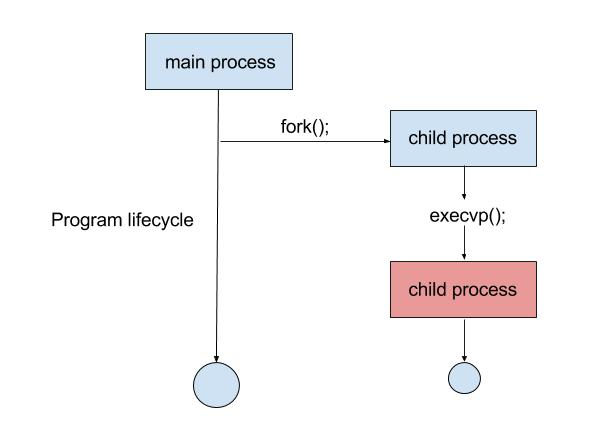
\includegraphics[width=0.5\textwidth]{Coding/execvp.jpg}
\end{center}

\begin{center}
    \tiny{Taken from \url{https://indradhanush.github.io/blog/writing-a-unix-shell-part-2/}}
\end{center}


\end{frame}

\begin{frame}
{\centerline{Ancestors of Virtual Environments}}
\begin{itemize}
    \item Code for executing a command in the shell
    \item Notice all the different kind of \texttt{execs}
\end{itemize} 
\begin{center}
    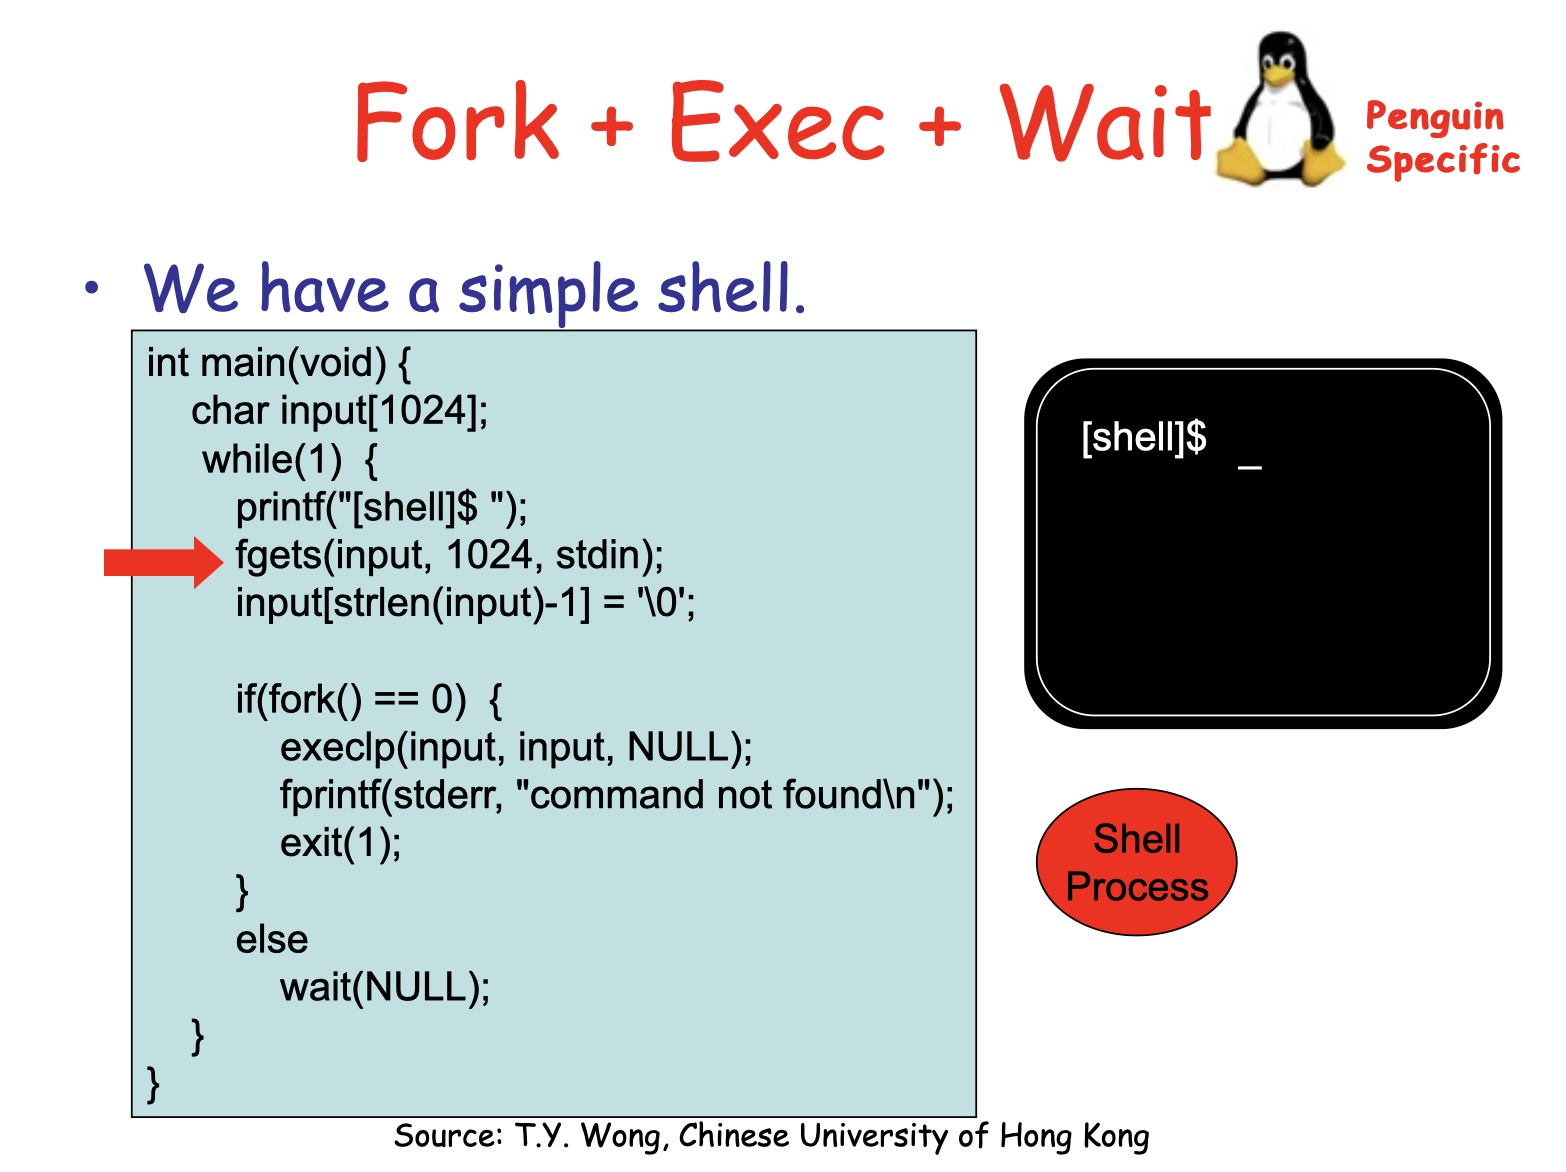
\includegraphics[width=0.6\textwidth]{Coding/forkExec.jpg}
\end{center}

\begin{center}
    \tiny{Taken from \url{https://slideplayer.com/slide/4999027/}}
\end{center}


\end{frame}

\begin{frame}
{\centerline{Remember the structure of a Python code}}
\begin{itemize}
    \item The ``executable'' of Python is not a single \texttt{a.out} that encloses (in theory) all the required libraries
    \begin{itemize}
    \item It requires a whole set of packages to load at run time
\end{itemize} 
    \item Therefore, it is not enough to have a ``specialized'' environment with suitably set environment variables
    \begin{itemize}
        \item The ``environment'' for a program now includes also a set of specific versions of specific packages
    \end{itemize} 
    \item Different programs need different environments
\end{itemize} 

\end{frame}

\begin{frame}
{\centerline{VirtualEnv and VENV}}
\begin{itemize}
    \item VirtualEnv \url{https://sourabhbajaj.com/mac-setup/Python/virtualenv.html}
    \item venv \url{https://www.studytonight.com/post/python-virtual-environment-setup-on-mac-osx-easiest-way}
\end{itemize} 

\end{frame}



\begin{frame}
{\centerline{Creating a Virtual Environment in PyCharm}}
\begin{itemize}
    \item 1. Click on the settings button
\end{itemize} 
\begin{center}
    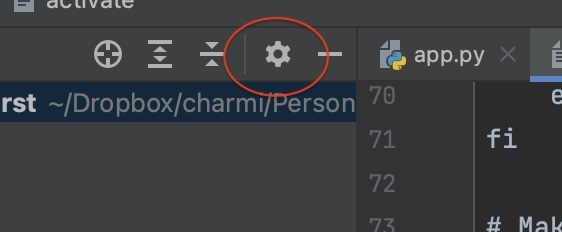
\includegraphics[width=\textwidth]{Coding/PyCharm.Settings.jpg}
\end{center}
\end{frame}

\begin{frame}
{\centerline{Creating a Virtual Environment in PyCharm}}
\begin{itemize}
    \item 2. Edit Scope
\end{itemize} 
\begin{center}
    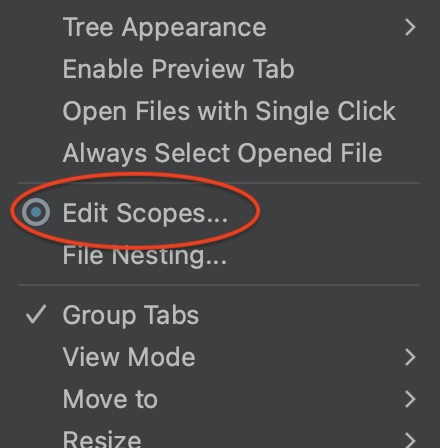
\includegraphics[width=0.5\textwidth]{Coding/PyCharm.EditScope.jpg}
\end{center}
\end{frame}

\begin{frame}
{\centerline{Creating a Virtual Environment in PyCharm}}
\begin{itemize}
    \item 3. Select the project
\end{itemize} 
\begin{center}
    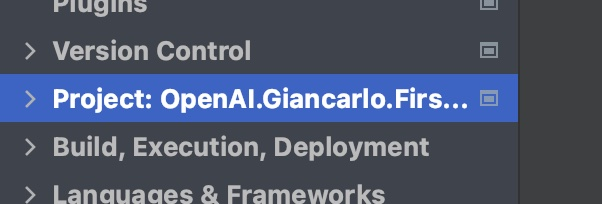
\includegraphics[width=0.6\textwidth]{Coding/PyCharm.Project.jpg}
\end{center}
\end{frame}

\begin{frame}
{\centerline{Creating a Virtual Environment in PyCharm}}
\begin{itemize}
    \item 4. Select Python Interpreter
\end{itemize} 
\begin{center}
    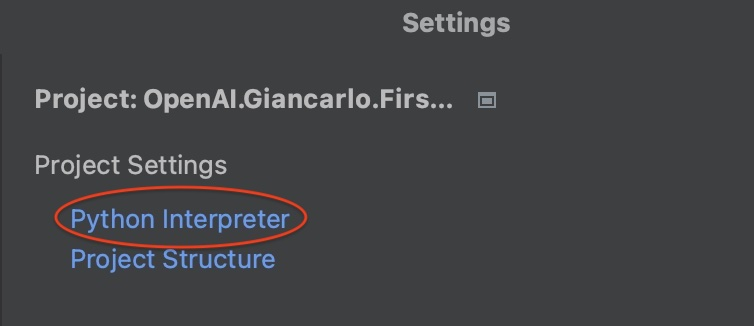
\includegraphics[width=\textwidth]{Coding/PyCharm.PhytonInterpreter.jpg}
\end{center}
\end{frame}

\begin{frame}
{\centerline{Creating a Virtual Environment in PyCharm}}
\begin{itemize}
    \item 4. Add Local Interprenter
\end{itemize} 
\begin{center}
    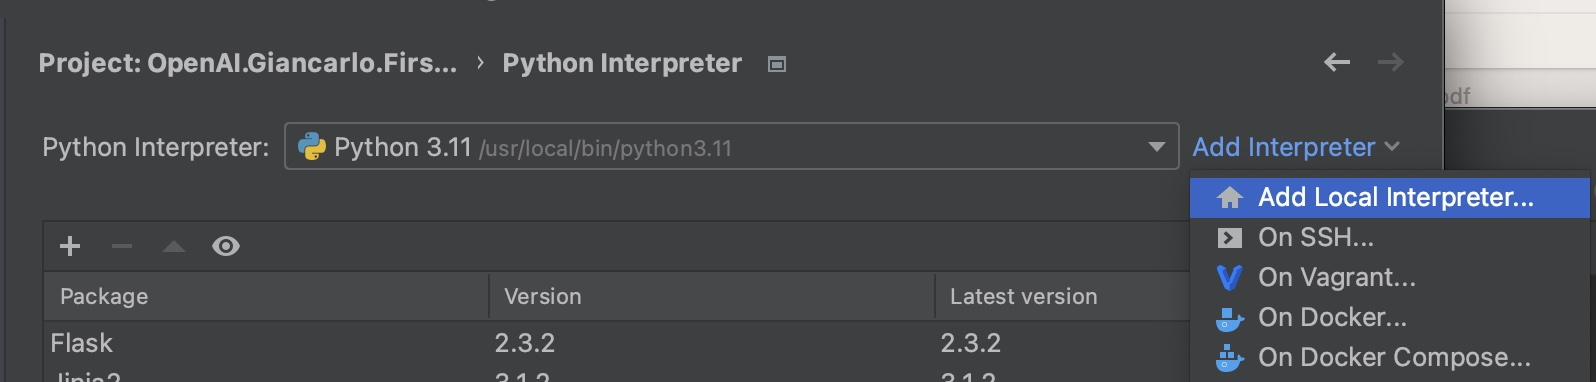
\includegraphics[width=0.8\textwidth]{Coding/PyCharm.AddLocalInterpreter.jpg}
\end{center}
\end{frame}

\begin{frame}
{\centerline{Creating a Virtual Environment in PyCharm}}
\begin{itemize}
    \item 5. Select the Virtual Environment and identify an empty directory
\end{itemize} 
\begin{center}
    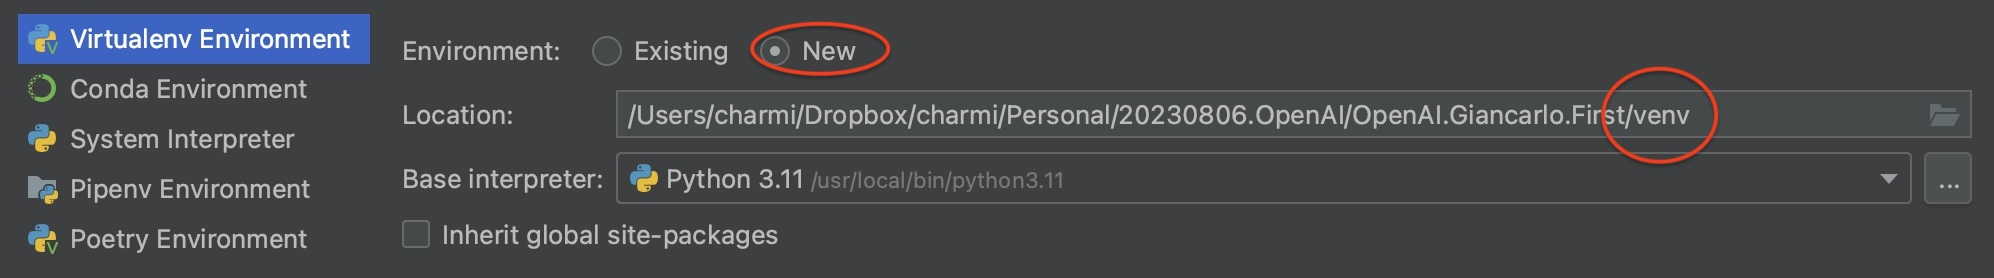
\includegraphics[width=\textwidth]{Coding/PyCharm.VirtualEnvironment.jpg}
\end{center}
\end{frame}

\begin{frame}
{\centerline{Creating a Virtual Environment in PyCharm}}
\begin{itemize}
    \item 6. Set the environmental variables (for using OpenAI key) 
    \begin{itemize}
    \item 6.1 Open the panel
    \end{itemize} 
\end{itemize} 
\begin{center}
    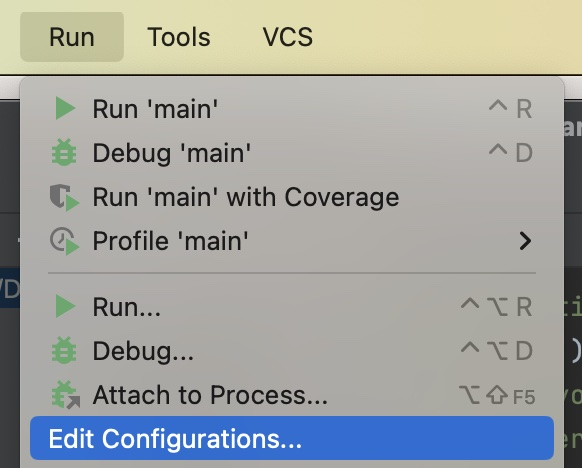
\includegraphics[width=0.6\textwidth]{Coding/PyCharm.RunEditConfigurations.jpg}
\end{center}
\end{frame}

\begin{frame}
{\centerline{Creating a Virtual Environment in PyCharm}}
\begin{itemize}
    \item 6. Set the environmental variables (for using OpenAI key) 
    \begin{itemize}
    \item 6.2 Select the environmental variables
    \end{itemize} 
\end{itemize} 
\begin{center}
    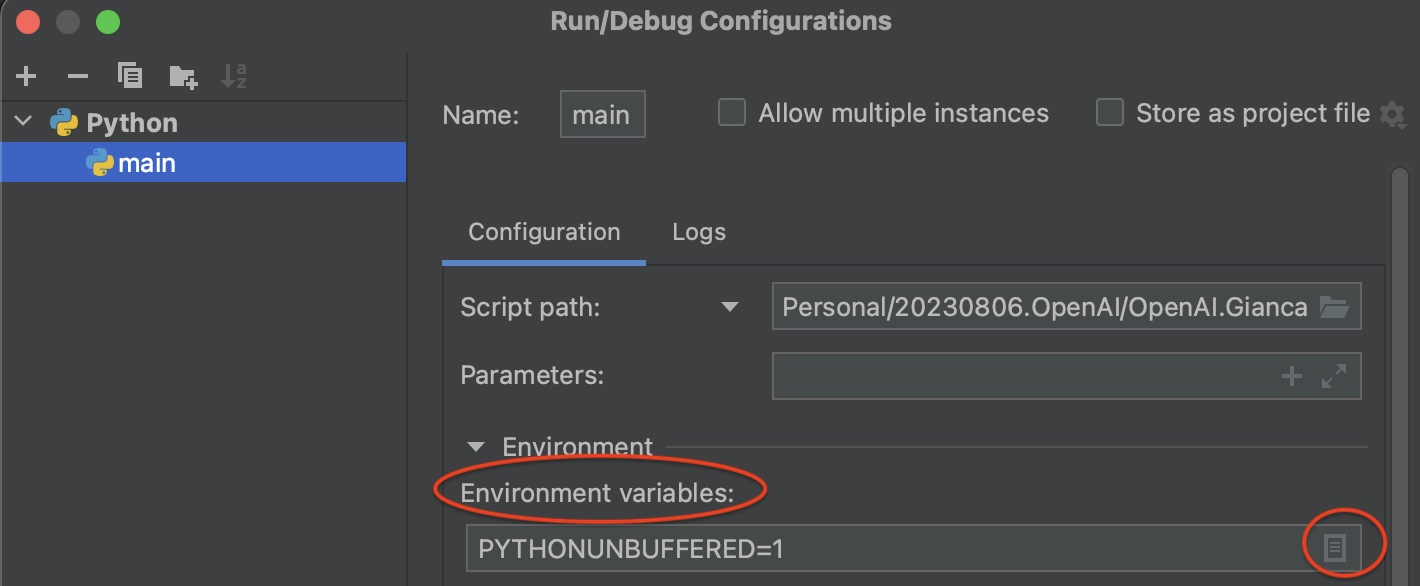
\includegraphics[width=1\textwidth]{Coding/PyCharm.EnvironmentalVariables.jpg}
\end{center}
\end{frame}

\begin{frame}
{\centerline{Creating a Virtual Environment in PyCharm}}
\begin{itemize}
    \item 6. Set the environmental variables (for using OpenAI key) 
    \begin{itemize}
    \item 6.3 Add an environmental variable
    \end{itemize} 
\end{itemize} 
\begin{center}
    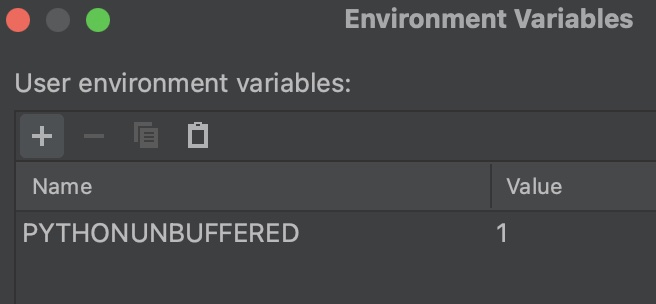
\includegraphics[width=0.9\textwidth]{Coding/PyCharm.AddEnvironmentalVariable.jpg}
\end{center}

\end{frame}

\begin{frame}
{\centerline{Creating a Virtual Environment in PyCharm}}
\begin{itemize}
    \item 6. Set the environmental variables (for using OpenAI key) 
    \begin{itemize}
    \item 6.4 Set the environmental variable
    \end{itemize} 
\end{itemize} 
\begin{center}
    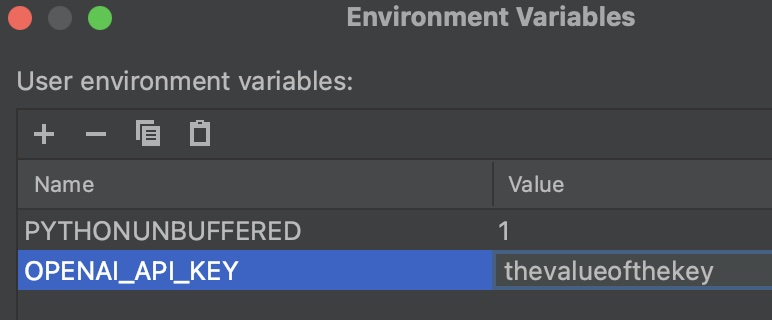
\includegraphics[width=0.9\textwidth]{Coding/PyCharm.SpecifyEnvironmentalVariable.jpg}
\end{center}
\begin{itemize}
    \item Note: The environmental variables can be set in the command line with the usual export mechanism \\ \texttt{export OPENAI\_API\_KEY=thevalueofthekey}

    \end{itemize} 

\end{frame}








\begin{frame}
{\centerline{Flask}}
\begin{itemize}
    \item To have simple web based applications -- inversion of control
\end{itemize} 
\begin{center}
    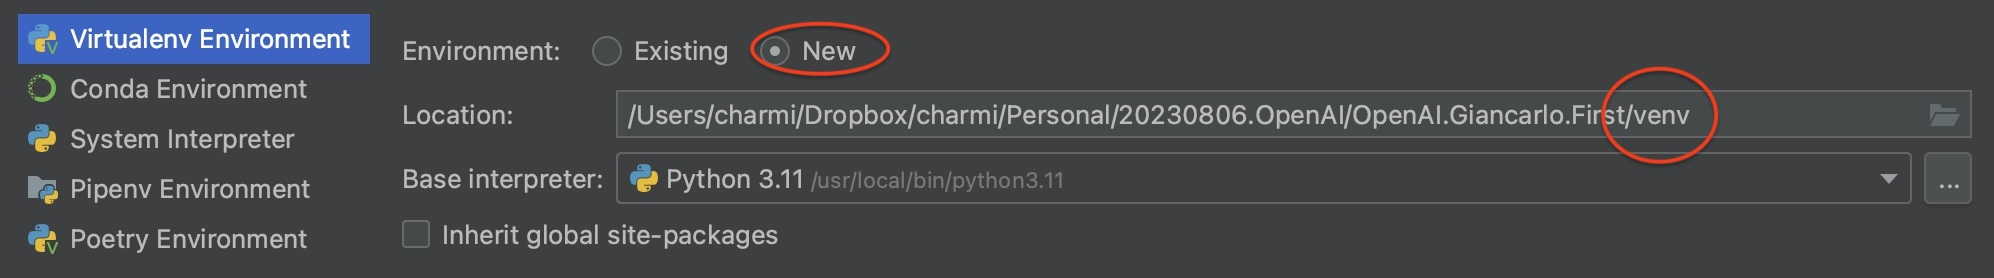
\includegraphics[width=\textwidth]{Coding/PyCharm.VirtualEnvironment.jpg}
\end{center}
\end{frame}


\begin{frame}
{\centerline{Coding in ChatGPT}}
\begin{itemize}
    \item Quickstart from the manual
    \item Understanding the code
    \item Extending the example
\end{itemize} 
\end{frame}

\begin{frame}
{\centerline{Chat Completion}}
\begin{itemize}
    \item Discussion on Chat Completion
    \item \url{https://platform.openai.com/docs/guides/gpt/function-calling}
    \item \url{https://platform.openai.com/docs/api-reference/chat}
\end{itemize} 
\end{frame}

\begin{frame}
{\centerline{Function Calling}}
\begin{itemize}
    \item Discussion on Function Calling
    \item \url{https://platform.openai.com/docs/guides/gpt/function-calling}
    \item \url{https://github.com/openai/openai-cookbook/blob/main/examples/How_to_call_functions_with_chat_models.ipynb}
\end{itemize} 
\end{frame}


\begin{frame}
{\centerline{Questions?}}
\vspace{1cm}
\begin{center}
    \LARGE{End of the lectures on ChatGPT.}
\end{center}

\end{frame}


\end{document}
